\chapter{Production Cost Analysis}
\label{ch:costanal}
%not prodcostanal, name has been changed later on, leave costanal as it has been used everywhere already. Next time make it with underscores as was the convention

The production cost of an aircraft comes from multiple aspects, to combine the results of these aspects a trade-off has been made presented in \autoref{sec:subtradcost}. The cost has been split up into five different categories: manufacturing cost, material cost, mechanism cost, power \& propulsion cost, and influence of weight on cost. The reason behind this division, the assigned weights and a brief explanation on the different categories will be provided in \autoref{sec:costcrit}. The production cost and layout of a conventional plane, scaled to the average weight of the concepts, are taken as a nominal value. The production cost of the nominal value will be estimated in \autoref{sec:nomval}. To do the trade-off with respect to cost, the concepts will be compared to this nominal value in \autoref{sec:conanal}. In this way, it is possible to assess if the costs of the concepts will be higher or lower than the nominal production cost.   

\section{Cost Trade-off}
\label{sec:subtradcost}
In this section, the cost trade-off will be presented and the results will be discussed. The grading system will also be described.

\subsection{Summary}
The trade-off table can be seen in \autoref{tab:costsubtradja}. The trade-off will provide the reader with an overview that visualises the result of all categories of costs and its corresponding weights.


\begin{table}[H]
    \centering
    \caption{Cost sub trade-off}
    \label{tab:costsubtradja} %please use your own label when you copy it!
    \begin{tabular}{r|>{\centering}p{2.5cm}:>{\centering}p{1.5cm}:>{\centering}p{1cm}:>{\centering}p{3cm}:>{\centering}p{2cm}|c}
    \textbf{Concept \rotatebox{90}{\hspace{0.5cm}Criterion}}    & 
    \rotatebox{90}{\textbf{Manufacturing}}                      &
    \rotatebox{90}{\textbf{Material}}                           & 
    \rotatebox{90}{\textbf{Mechanism}}                          & 
    \rotatebox{90}{\textbf{Power \& Prop}}                      & 
    \rotatebox{90}{\textbf{Mass}}                             &
    \rotatebox{90}{\textbf{Outcome}} 
    \\ \midrule
    Tailsitter      & + +   & + +   & - -   & - -   & 0     & 50\% 
    \\\hdashline
    Tandem          & -     & -     & -     & +     & -   & 36.25\% 
    \\\hdashline
    Prandtl Box     & - -   & - -   & +     & +     & + +   & 50\% 
    \\\hdashline
    Tiltrotor       & 0     & - -   & - -   & -     & - -     & 20\% 
    \\\hdashline
    Winged Quad.    & 0     & 0     & 0     & 0     & +   & 55\% 
    \\ \midrule\midrule
    Weight          & 25    & 15    & 10    & 30    & 20    &  
    \end{tabular}
\end{table}

With an outcome of 55\%, The Winged Quadcopter has the highest score of all concepts with respect to costs. The Winged Quadcopter scores no minuses on the general criteria since the configuration of this concept is very similar to the nominal aircraft, one plus is scored on the influence of weight. There are some differences in the configuration of The Winged Quadcopter, e.g., the extra beams to hold the propellers but these differences are negligible with respect to cost. Its low weight makes the concept have a high resulting score. 
The second best concepts, with only 5\% less than the first one, are The Tailsitter and The Prandtl Box. The Tailsitter has low costs for manufacturing and material since it is a flying wing. However, using a single, engine with counter-rotating propellers for propulsion is expensive and requires expensive mechanisms for control. The Prandtl Box also scores high while having a complex wing which is very difficult to manufacture and a fuselage requiring substantial structural strength; its weight gave it its high score.

The next concepts have a score which differs a lot from the first three ones. This means that these concepts are clearly more expensive than the previous three. The Tandem has minuses for everything except the propulsion sub-criterion. It scores good on propulsion because of its four engines. The UAV with the lowest score is The Tiltrotor scoring minuses on every sub-criterion except for manufacturing costs. 

In short, The Tailsitter, The Prandtl Box and The Winged Quadcopter are the obvious winners of the cost trade-off. The other concepts have clear disadvantages with respect to cost. 

\subsection{Grading System}

The trade-off grading has been done by assigning pluses, minuses and zeroes to every concept on multiple cost criteria. In this way, the table gives a clear overview of what the concepts score relatively to each other and to the nominal value for each sub-criterion. \autoref{tab:costweight} shows the explanation behind the grading system used. 

\begin{table}[H]
\centering
\caption{Definition of cost grading system}
\label{tab:costweight}
    \begin{tabular}{rl}
        \toprule
        \textbf{Rating}           & \textbf{Meaning}
        \\ \midrule
         + +            & Excels          
        \\ \hdashline
        +               & Better
        \\ \hdashline
         0          & Average 
        \\ \hdashline
          -           & Worse 
        \\ \hdashline
         - -    & Bad  %how about this? Poor is also an option, or erroneous; uh uh, and unacceptable is unacceptable in this context, don't delete the comment x_x
        \\ \bottomrule
    \end{tabular}
\end{table}

To calculate the outcome of the trade-off, each criteria score will be multiplied with the corresponding weight, with each '+' being equal to 1 and each '-' being equal to -1. The highest possible score would be 200 while the lowest possible score would be -200. For ease, this scoring should be scaled from 0 to 100. In order to do this, the outcome shall be divided by four (to reduce the range from [-200,200] to [-50,50]). Finally, 50 will be added to this number to bring the range to [0,100].

\section{Cost Criteria}
\label{sec:costcrit}
This section will describe and discuss the different cost criteria used in the trade-off, in \Cref{sec:mancost,sec:matcost,sec:mechcost,sec:powercost,sec:weiginflcost}. The reasoning behind the assigned weights of the criteria will be explained in \autoref{subsec:critweightcost}. 

\subsection{Manufacturing Costs} 
\label{sec:mancost}
The manufacturing costs depend greatly on the complexity of the aircraft. The production of a more complex aircraft requires more man-hours, a bigger facility, more material, better tools or simply more time to be produced; which all cost money. To know what the share of each aspect is in the total manufacturing cost, a brief analysis has been made. \autoref{tab:manucosts} shows the percentage of costs for labour, materials and other costs of the manufacturing process\footnote{https://dspace.mit.edu/bitstream/handle/1721.1/16871/51679351-MIT.pdf?sequence=2, Accessed 11-05-2017}.


This table shows that most of the manufacturing cost, around 41\%, goes into labour. The 'other' costs take up around 26\% of the manufacturing cost and 33\% goes to the material cost. In this trade-off, the manufacturing cost includes the labour and other cost. The material cost will be a separate criterion which will have a weight that is approximately half the weight of the manufacturing cost. 

\begin{table}[H]
    \centering
    \caption{Percentages of manufacturing costs}
    \begin{tabular}{cccc}
    \toprule
         & Labour & Materials & Other \\ \midrule
    \% of costs     & 41 & 33 & 26 \\
    \bottomrule
    \end{tabular}
    \label{tab:manucosts}
\end{table}

The first aspect of the manufacturing cost is the 'other costs' which are costs for quality assurance, and the required tools and machines. These will be seen as facility related costs. The facility needed depends on a few factors: machines, tools, complexity of assembly, and complexity of the concept. The machines and tools needed differ for each concept: one might need a machine which can bend sheets to make wings with double curvature while other concepts might need big and complex tools such as moulds for laminating the wings. The complexity of assembly also plays a role: a concept might require assembly of different parts of the wings, while other concepts are able to build the wing in one piece. When the complexity of the assembly increases, the required man-hours  and amount of assembly lines also increase.

The second aspect of the manufacturing costs is the amount of man-hours needed to manufacture the UAV. Time is money, hence the longer the process, the more it will cost. To assess the time needed to manufacture the UAV, the concepts will be analysed on how complex they are.

\subsection{Material Costs} 
\label{sec:matcost}

A higher amount of material or using a more expensive material means it will have a higher cost. Even though material costs are actually a part of manufacturing costs, the decision has been made to separate these two aspects because the material costs may have a great influence on the price of the UAV. If these two aspects were put together, a UAV with a low material cost but complex shape, hence high manufacturing cost, will eventually lead to a medium value for the total cost, not showing which aspect is expensive or not. In this case, using two separate aspects is more insightful. 

To assess whether or not the concept will have high material costs, rough estimates need to be made of how big the concept will be and how it will handle stresses in comparison to the nominal value. If, for example, a UAV has heavy engines on the tip of a wing, strong and heavy wingboxes will be necessary to support the structure. Hence, the material cost will be larger than for a conventional aircraft. Another example is that a concept might have a lot of surface area, increasing the material needed to build the concept which will increase the cost.

\subsection{Mechanism Costs}
\label{sec:mechcost}

When dealing with Hybrid UAVs, the designs may have a lot of movable parts. For this reason the concepts will be analysed for the extent to which they rely on complex, hence expensive mechanisms: will they have rotatable engines, movable wings or other moving parts. To move these parts, actuators will be needed and integrated into the design. These actuators will also have influences on the manufacturing cost and power cost, but those influences will be assessed in the respective criteria. In this criterion, purely the costs of the mechanism will be analysed.

Not only the movable parts unique to a specific Hybrid UAV will be analysed for these costs, but also the control surfaces. Possibly, one concept will have less control surfaces than a conventional aircraft, hence having less mechanism costs, or have a complicated swash plate in order to control the UAV.

\subsection{Propulsion \& Power Costs} 
\label{sec:powercost}

The Propulsion \& Power cost is a big cost with respect to the total cost of the UAV. Also, the propulsion cost may differ significantly between the concepts depending on the number of engines. Since propulsion and the power needed for propulsion are closely related to each other, these two criteria are grouped together. 

\subsection*{Propulsion Costs}
\label{sec:propcost}
Within propulsion costs there are two things that could be taken into account: the propeller costs and the engine costs. It can be assumed that the propeller cost doubles when the amount of propellers double, but the cost for the propellers are negligible in comparison with the engines costs.To find the cost of the engines, some literature study must be made to find the price of certain engines, the ratio of cost over power, the ratio of cost over torque and how the price relates to the number of engines used. 

The case of vertical climb is analysed since this is the flight phase where most power is needed.
The first step taken in order to estimate the costs of the propulsion system was to find an equation for the power required during vertical climb. Use is made of \autoref{eq:goodpow}\footnote{\url{http://s6.aeromech.usyd.edu.au/aerodynamics/index.php/sample-page/aircraft-performance/hoverclimbdescent-analysis/}, Accessed 18-05-2017} 

%which is derived in Appendix \autoref{chap:preq}.

\begin{equation}\label{eq:goodpow}
    P_{req} = T \cdot \left( \frac{V_{c}}{2} + \sqrt{ \left( \frac{V_{c}}{2} \right) ^2 + \frac{T}{2 \rho A}} \right)
\end{equation}

The equation shows that the power required depends on the climbing speed, the required thrust, the air density and the surface area of the propellers.  One can see that the thrust needed in order to climb vertically at a certain acceleration is equal for all concepts since it is assumed that the mass is equal for all concepts. It can also be assumed that the total propeller area is the same for every concept. Furthermore, the density at 2000m is taken in this equation. From this it can be concluded that the power required to climb at a certain acceleration and velocity will be the same for all concepts with any number of engines.

Two other parameters related to power play an important role when looking at engines: the torque and Rounds Per Minute (RPM). These two values make the difference between a cheap engine and an expensive engine. The cost of the engine will be higher for engines with higher torque and with lower RPM, since power is equal to torque times RPM.  

The airflow  over the propeller cannot be supersonic because the vibrations coming from the shock waves could destroy the propeller. Therefore, the tip velocity of the propeller will determine the maximum allowable RPM for a given propeller. The maximum RPM follows from \autoref{eq:tipspeed}.

\begin{equation}\label{eq:tipspeed}
\begin{aligned}
    %\text{Knowing the radius, r,}&\text{ from the required propeller area:}\\
    V_{max} =& 0.9 \cdot a \\
    \omega_{max} =& \frac{V_{max}}{2 \pi r} \Big[\frac{rad}{s}\Big] \\
    RPM =& \frac{V_{max}}{2 \pi r} \cdot \frac{60}{2 \pi} \Big[\frac{rev}{min} \Big]
\end{aligned}
\end{equation}

The maximum tip velocity has been taken as Mach 0.9 in order to prevent local shock waves to occur too. Knowing the maximum RPM, it is possible to calculate the minimum torque in order to generate the required power:

\begin{equation}\label{eq:powtor}
    \tau = \frac{P}{\omega}
\end{equation}

Knowing the maximum possible RPM and minimum torque to get the required power, it is possible to look at the costs of the propulsion system for engines with different torques and power settings. Statistical data was collected in order to find the relation between power and cost, and torque and cost in \autoref{fig:costvspow} and in \autoref{fig:costvstor} respectively. Both graphs show that the relation with cost is linear for power and for torque. It is assumed that the trend line for cost vs power and torque intersects at the origin.

%\begin{comment}
\begin{figure}[htb]
    \centering
    \begin{subfigure}[b]{0.45\textwidth}
        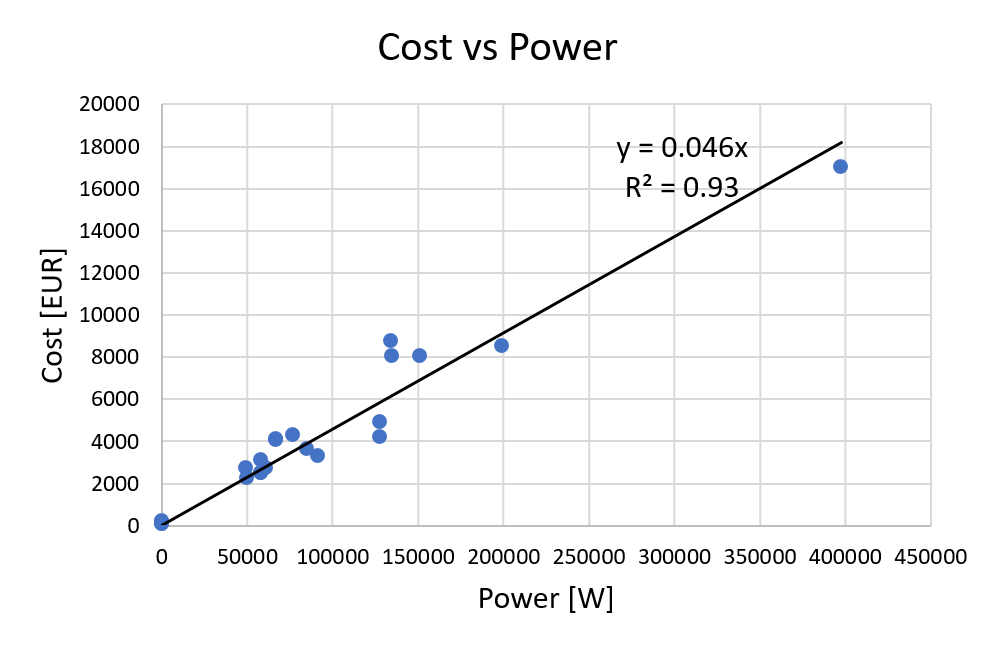
\includegraphics[width=\textwidth]{CostAnalysis/Figures/costvspower.PNG}
        \caption{Cost versus power relation}
        \label{fig:costvspow}
    \end{subfigure}
    \begin{subfigure}[b]{0.45\textwidth}
        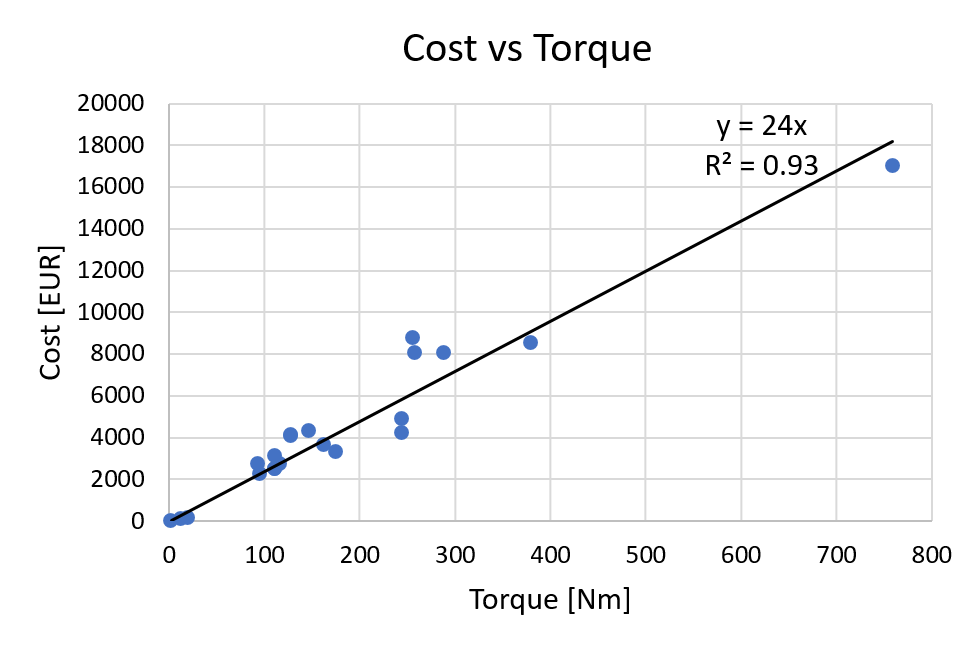
\includegraphics[width=\textwidth]{CostAnalysis/Figures/costvstorque.PNG}
        \caption{Cost versus torque relation}
        \label{fig:costvstor}
    \end{subfigure}
    \caption{Cost trendlines for torque and power}
    \label{fig:costtrendlines}
\end{figure}
%\end{comment}


When considering that the power required to climb is the same for each concept, one may think that the cost will be equal too. That is not the case since the tip velocity limits the RPM hence a minimum torque is required. In some cases, an engine with this limiting amount of torque may be more expensive than the value that can be seen for the power required. \autoref{fig:clearance} shows the total cost of engines depending on the propeller's area for different numbers of engines. An acceleration of 4 $\frac{m}{s^2}$, a $V_c = 4$ $\frac{m}{s}$ and a mass of 52 kg is taken. The cost is taken versus the propeller area because it is the same for different numbers of engines and it also resembles the radius of a specific number of engines which limits the maximum RPM. When having one propeller, a larger radius is needed in order to have the same total propeller area as a two/four propeller UAVs. This means the maximum allowable RPM will be lower, requiring a larger torque to achieve the amount of power. The power cost constraint will stay the same for different amounts of propellers since it only depends on the area which is the same for all number of engines.


\begin{figure}[htb]
    \centering
    \begin{subfigure}[b]{0.53\textwidth}
        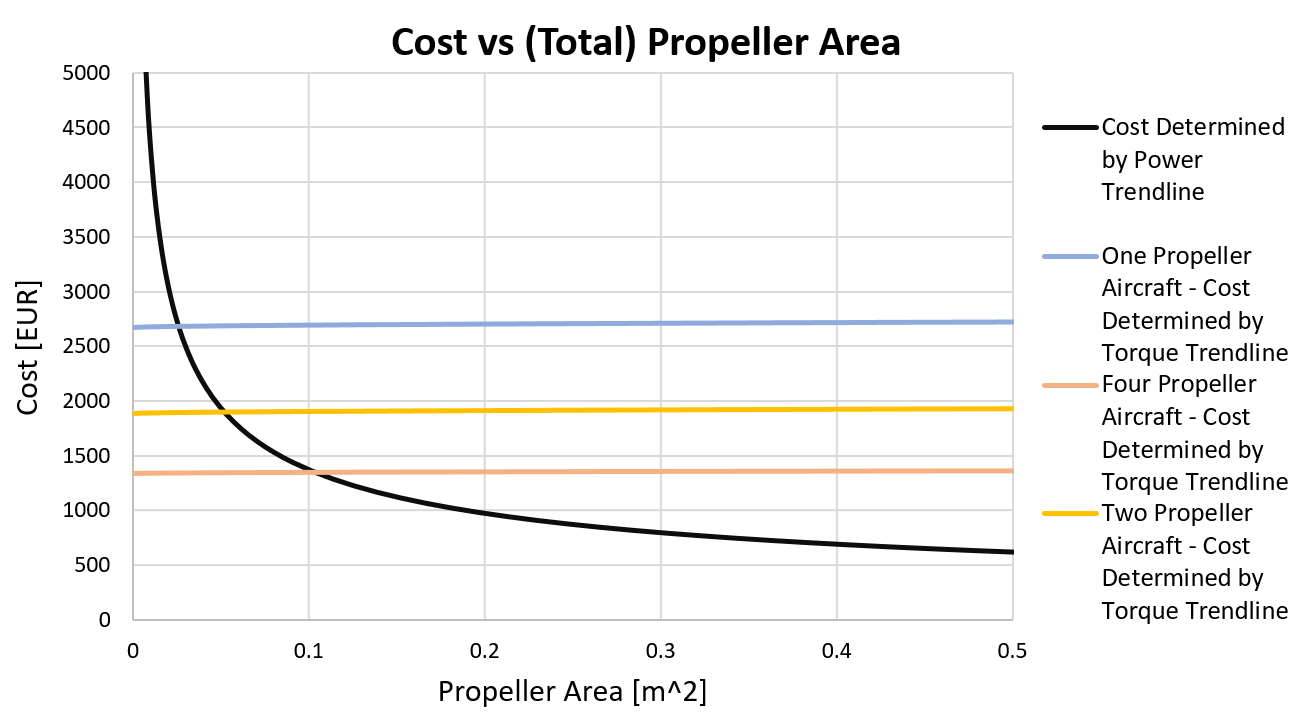
\includegraphics[width=\textwidth]{CostAnalysis/Figures/costvsarea2.PNG}
        \caption{cost vs propeller area}
        \label{fig:clearance}
    \end{subfigure}
    \begin{subfigure}[b]{0.45\textwidth}
        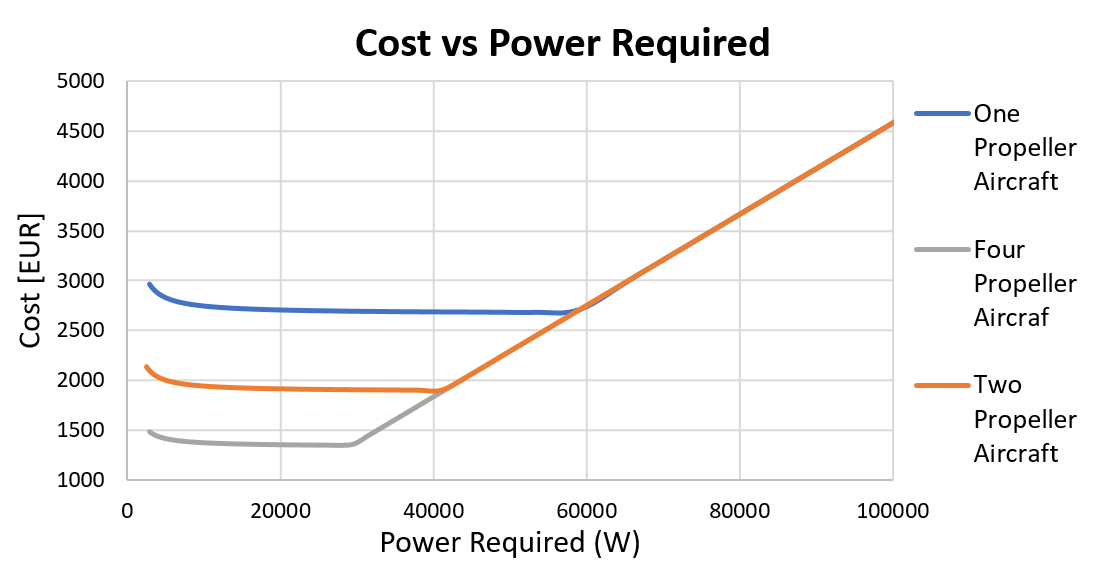
\includegraphics[width=\textwidth]{CostAnalysis/Figures/costvspower3.PNG}
        \caption{Cost versus power}
        \label{fig:costvspower}
    \end{subfigure}
    \caption{Cost graphs for one two and four engines}
\end{figure}

What can be seen in \autoref{fig:clearance} is that the cost is first determined by a power constraint and when the propeller area becomes larger it is determined by the minimum torque required. The point where the lines cross, is the point where the cost determined by the torque starts to take over. While the power required decreases vastly for an increase in propeller area, the torque required is increasing ever so slightly. \autoref{fig:costvspower} shows the highest cost for each UAV with respect to the power required.


It is interesting to notice that for a high power required, which corresponds to a small propeller area, the costs are the same for different numbers of engines. The point where the torque determined cost meets the power determined cost is the point with minimal cost. When the power required gets even smaller, the cost starts to increase heavily. This is due to the required minimum torque which is increasing to keep the required power while the angular velocity is decreasing due to the supersonic constraints. 

Going back to the effect of having multiple engines in comparison to one, the results show that it is more cost efficient to have multiple engines. A four time increase in engines may decrease the cost by half when the torque limits the cost (left side of the graph). When looking at the side where power limits the cost, having multiple engines or only one engine doesn't change the cost of the engine. So eventually, it all leads to the size of the propellers which determines the area, which determines the required power. Having them too small will mean the power required is very high, which means the UAV will have expensive engines due to the power determined cost. Having big propellers will mean that the torque needs to be big because of the low angular velocity required to prevent local sonic flow conditions, causing the cost to increase as well. 

When assuming that the power required is kept on the left side of the graph, then a four times increase in number of engines leads to a two times decrease in cost. If the total power remains the same for four engines, the power per engine will be one fourth. Also, having four engines instead of one means that the required propeller radius will be halved for each of the propellers. Looking at \autoref{eq:prooftor}, it is shown that the angular velocity will be doubled for a halved radius. The subscripts 'four' and 'one' clarify how many engines the UAV has.

\begin{equation}\label{eq:prooftor}
\begin{aligned}
    \omega_{four} = \frac{V}{2 \pi r_{one}} = \frac{V}{\pi r_{four}} = 2 \omega_{one}
\end{aligned}
\end{equation}

Using this relation to calculate the required torque yields:

\begin{equation}\label{eq:prooftor2}
    \tau_{tot_{four}} = \frac{P}{\omega_{four}} = \frac{P}{2\omega_{one}} = \frac{1}{2} \frac{P}{\omega_{one}} = \frac{1}{2}\tau_{tot_{one}}
\end{equation}

The total torque on a four-engine aircraft will be halved. Seeming that the torque determined cost is linear, the cost will also be halved. The relationship between number of engines and torque determined cost is: an N times increase in engines is $\sqrt{N}$ decrease in cost.


\subsection*{Power Costs}

The more power needed the more energy storage will be required. No definite choice has been made whether the Hybrid UAV will be using electric propulsion or not, but even when the propulsion would be combustion based, batteries will be needed. These will be needed to start the aircraft, rotate certain parts and move the mechanisms. Since batteries have a high price per kWh (around 175 euro / kWh)\footnote{https://electrek.co/2017/01/30/electric-vehicle-battery-cost-dropped-80-6-years-227kwh-tesla-190kwh/, Accessed 15-05-2017} the amount of energy needed will play a big role in the costs trade-off. 

To make a rough estimate of the cost of the power subsystem, a look needs to be taken in the subsystems that are using that power: the propulsion system (especially if electric), the mechanisms, the instruments and the Central Processing Unit (CPU). The propulsion system takes up the most power. To distinguish battery cost for the different concepts, the concepts will be analysed on how efficient they can fly. Hence, using less energy and a smaller amount of extra subsystems that need power. For example, when using a lot of mechanisms, such as rotating wings, more power is needed and the cost will be higher. Also, fans are more efficient than propellers when flying under 160 km/hr. Therefore, fans use less power making the power subsystem cheaper\footnote{http://www.esotec.org/hbird/HTML/DuctMyths\_F.html, Accessed 22-05-2017}.


\subsection{Weight Influence on Costs}
\label{sec:weiginflcost}

The weight of the concepts will greatly influence the production cost because weight is indirectly involved with all aspects of cost. To analyse the effects of cost, a look will be taken into each sub-criterion to find out how weight affects it. For the analysis of the other sub-criteria, the weight of the concepts will be considered as equal. In this way, the differences between the concepts on one sub-criterion can be found without interference of the other factors.

\paragraph{Manufacturing Costs} When the weight of a concept increases, the manufacturing cost goes up too. Not only will the facility needed to build the aircraft increase in size, but all tooling, machines and further equipment (e.g. moulds) will need to be bigger and thus cost more.

\paragraph{Material Costs} When the concept weighs more, there will be stronger forces on the aircraft: more lift, more drag, more thrust, stronger bending moments, and so on. To withstand these forces the structure needs to be stronger, requiring more structural components, thicker material or stronger materials. Another increase in cost comes from the fact that there will be more lift needed to lift the aircraft in horizontal flight, which comes from larger surfaces (e.g. wings and tail planes). These will increase the surface area of the aircraft and more material will be needed.

\paragraph{Mechanism Costs} The only change in costs at the mechanisms is that bigger and more complex mechanisms may be needed to hold the weight of the aircraft. This extra cost is assumed to be not as much as the other increases.

\paragraph{Power \& Propulsion Costs} This group is most affected by weight. The extra weight will influence a lot of the aircraft, which all influences the amount of power  needed. It first starts with the thrust needed to fly the aircraft vertically. An increase in weight means more thrust is needed which in turn means that the engines need to provide more power. A bigger, heavier and more expensive engine will be the result. Some bigger propellers may also be needed, but this cost is negligible with respect to the engine. Due to the heavier engines, more power will be needed to power them, so bigger batteries are necessary. More power will also be needed to move certain parts with the same speed(e.g. rotating wings with The Tandem) due to the parts being heavier and having a bigger moment of inertia. Though this extra power required is negligible when comparing it to the extra power required for thrust.


\subsection{Criteria Weights}
\label{subsec:critweightcost}

Assigning weights to the criteria is an important part of doing a trade-off. To weigh the criteria correctly some literature study should be done on each. This has been done and can be found in \Cref{sec:mancost,sec:matcost,sec:mechcost,sec:powercost,sec:weiginflcost}. The most important criterion will be the power \& propulsion costs, this is because this aspect takes up a large percentage of production cost. This can be seen in \autoref{sec:powercost}, where the cost of the engines can go up to 10k EUR for a single propeller for a 100 kilogram UAV. Because of this important, the propulsion \& power costs will have a weight of 30. After propulsion, the manufacturing cost has the highest weight. When taking manufacturing and materials together as a group, they take up 40\% of the total production costs. The weight of manufacturing will be twice as large as that of materials, based on \autoref{tab:manucosts} in \autoref{sec:mancost}. Therefore, the manufacturing cost has a weight of 25\% and the material cost has a weight of 15\%. The mass has a weight of 20\%. The weight of the aircraft will increase the costs of all parts, hence why it is of such importance. The mechanism cost only has a weight of 10\%. Finally, the power \& propulsion cost gets a weigth of 30\%.


\section{Nominal Values}
\label{sec:nomval}

In order to perform the production cost trade-off, all concepts are compared to a nominal value. The nominal value is defined as a conventional fuselage-wing-tail aircraft with a mass of 52 kg, which is the average mass of the concepts. This nominal value was chosen because it contains the most important features of a hybrid UAV with respect to production and because the production of this concept is already generalised. Therefore, adding aspects to the non-conventional configuration, e.g. adding a mechanism or using a Prandtl box wing, will result in more production cost. When aspects are removed from the conventional production process, e.g. removing the tail, the production cost will be lower.

\begin{figure}[H]
    \centering
    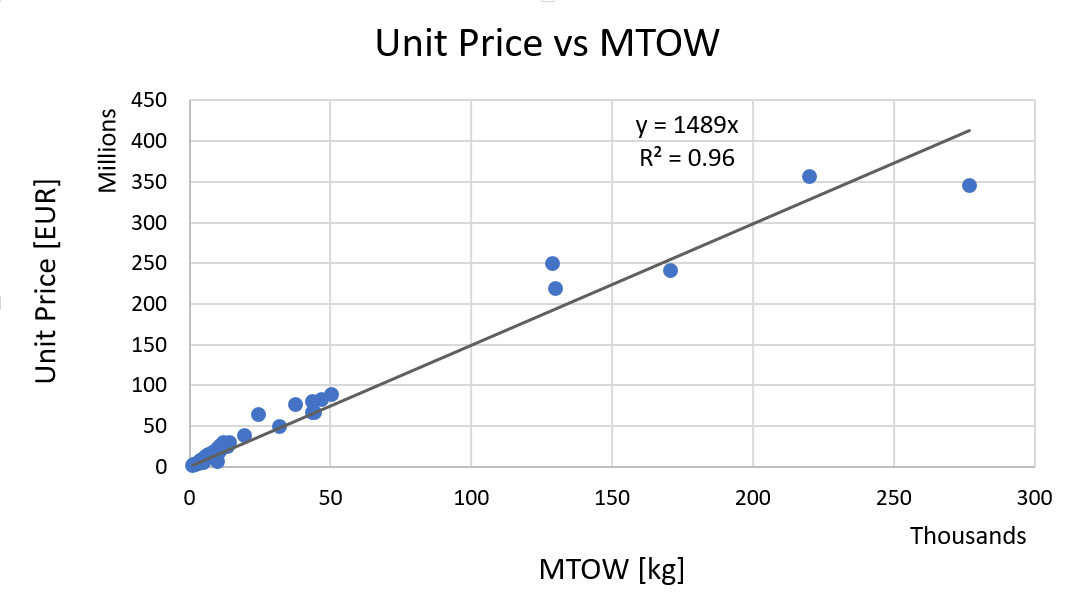
\includegraphics[width=0.6\textwidth]{CostAnalysis/Figures/Nomval}
    \caption{Relation between the unit price and the MTOW of conventional aircraft}
    \label{fig:nomvalgraph}
\end{figure}

The production cost of the nominal value is estimated in order to get a hunch of the magnitude of the cost. This is done by using statistical data of the nominal value: the conventional plane. In \autoref{fig:nomvalgraph}, the unit price of different aircraft is plotted against the Maximum Take-Off Weight (MTOW) of the aircraft. When a linear trend line, with intersecting point (0,0), is fitted to the data points, a relation is found between the unit price and the mass of the nominal value. Filling in the average mass of the Hybrid UAV concepts, being 52 kg, yields a unit price of around 77k EUR. Since there is a big difference in mass between conventional aircraft and the Hybrid UAV, one may wonder if this trend line can still be followed for masses in the order of 100 kg. This can be validated since aircraft of different mass categories, ranging from 1134 kg to 277000 kg, are used as data points while still having a very high $R^2$. \newline

Now, the unit price of the nominal value is estimated. However, the production cost is only a small part of the unit price. In general, the unit price consists of the profit, the development cost and the production cost. The profit per unit takes up around 5\% of the unit price \cite{costprofit}. The development cost per unit depends greatly on how many units are sold. Also the production cost per unit decreases with increasing amount of units sold. For the case of hybrid UAVs, it can be estimated that 80\% of the unit price goes to development cost since only few units are sold and many man-hours are spent into developing the concept. That leaves 15\% for the production cost. Using the unit prices estimated for the nominal value, a production cost of around 12k EUR is calculated.

\begin{figure}[H]
    \centering
    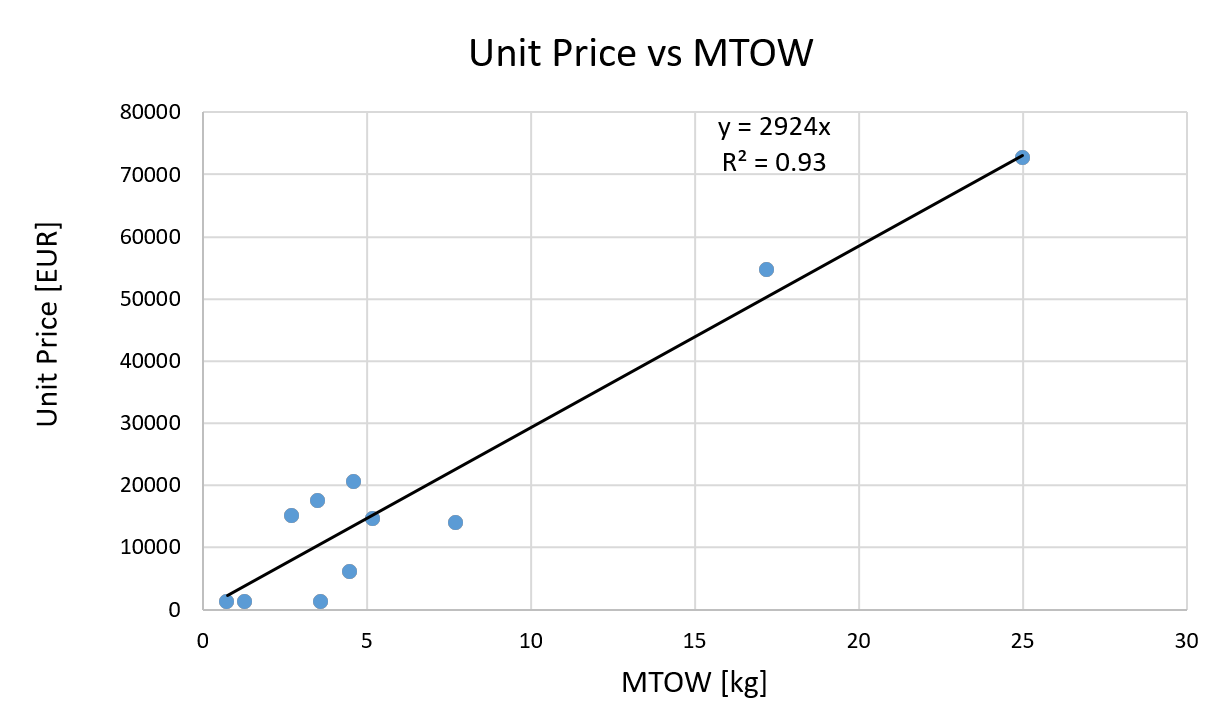
\includegraphics[width=0.6\textwidth]{CostAnalysis/Figures/CostEst}
    \caption{Relation between the unit price and the MTOW of hybrid and fixed wing UAVs}
    \label{fig:nomcost}
\end{figure}

A cost estimation for hybrid and fixed wing UAVs is also carried out in order to find out how the unit price of the nominal value will differ in price with an actual, similar UAV. In \autoref{fig:nomcost} the unit prices of hybrid and fixed wing UAVs are plotted against the MTOW. From the trend line, one can estimate a UAV of 52 kg to have a unit price of around 152k EUR. This number is significantly higher than the unit cost calculated with the conventional aircraft estimation, this can be explained by taking into account the non-recurring costs. The non-recurring cost per unit for aircraft will be much lower than  for UAVs since an aircraft will have much more units sold than UAVs which are typically designed for only one specific mission, e.g. killer drones, ambulance drones or surveillance drones. This means that for UAVs there will be more development cost per unit but also, to a lesser extent, more production cost. The production cost for UAVs will also be slightly higher than those of a conventional aircraft because UAVs generally include more features than a conventional aircraft, e.g. hovering capabilities or VTOL. From the unit price for a 52 kg UAV one can calculate that the production cost would be around 23k EUR. This estimation lies very close to the cost requirement stated by Avy.


\section{Concept Analysis}
\label{sec:conanal}
In this section, the five chosen concepts will be analysed for cost on five different criteria: the manufacturing cost, material cost, mechanism cost, power \& propulsion cost and weight influence on cost.  
\subsection{The Tailsitter}

\paragraph{Manufacturing Costs}\label{sec:tailmanu}

The Tailsitter scored two pluses in this category. The first reason is that it is missing a fuselage structure, this means that there is a big part not needed to be manufactured. In general, the fuselage takes up 28\% of the total manufacturing costs\footnote{https://ocw.mit.edu/courses/aeronautics-and-astronautics/16-885j-aircraft-systems-engineering-fall-2004/lecture-notes/pres\_willcox.pdf, Accessed 02-05-2017}. The next reason is the low complexity of The Tailsitter: it has no secondary curves. Because of this it is easy to manufacture seeming it does not need special tools and machines compared to the nominal value. Laminating and other processes that may be required can be done easily on these flat surfaces. The last dominating reason is that the assembly of this aircraft would be very simple. There are just three major parts in this aircraft (tailplane, engine and wing) which can be assembled without much difficulties.

There are also disadvantages: the first one being that the inside of the wing will be more complex because it will need more support structure than the nominal plane to carry all the loads. This will take up more time to manufacture, costing more man-hours. This disadvantage does not have as big of an impact as the advantages combined, causing The Tailsitter to keep its two pluses.


\paragraph{Material Costs}

Two pluses are scored by The Tailsitter for the material cost. The material costs will be lower than the nominal aircraft. The first reason is that there is no fuselage, skipping a lot of the materials required to keep such a structure to strength. The next reason is derived from the expected loading cases. The greatest forces that will be encountered by the Hybrid UAVs act when they are taking off, this aircraft however can handle this force pretty well. When this aircraft needs to take off, it will pull the whole aircraft by its nose, creating a pulling force on the structure. This pulling force can easily be absorbed by the structure because it will not create bending moments or other stresses besides the tension.

\paragraph{Mechanism Costs}

For mechanism costs, The Tailsitter scores two minuses. It has conventional control surfaces and no complex moving wings but the propellers are making the costs go up. The first reason for this is that the propellers are counter-rotating, requiring complex mechanisms which will be expensive to buy or manufacture. Besides this, the propulsion system will have a swash plate for control. This has a high cost which is not present in the nominal configuration\footnote{http://www.heli-factory.com/eng/accessories/taumelscheibe-heli-factory/index.php , Accessed 10-05-2017}$^,$\footnote{http://www.vortechonline.com/awparts/, Accessed 10-05-2017}.

\paragraph{Power \& Propulsion Costs}
The Tailsitter scores two minuses on power \& propulsion since it has only one engine with two counter rotating propellers. Using only one propeller is very cost inefficient, it costs twice as much as using four propellers as is explained in \autoref{sec:propcost}. If one engine is used, the engine costs 4k EUR calculated for a mass of 52 kg. Furthermore, the counter rotating propeller is 9-17\% more efficient but also has 27\% more acquisition cost than regular propellers \cite{vanderover}. This will make the propulsion part of the cost very expensive. The power subsystem costs less since the propellers are more efficient. Hence, less power is required to provide the same thrust.

\subsection{The Tandem}

\paragraph{Manufacturing Costs} The Tandem is expected to have high manufacturing costs, causing it to score one minus in this category. The wings of this aircraft have a complex bend at the end, which will require extra tooling and machines to manufacture it. This complex bend will also require more man-hours. Another reason is that the assembly will be complex because each wing has to be attached to the fuselage separately via the mechanisms.

\paragraph{Material Costs} This aircraft scores another minus on material cost. The reasoning behind this is that it needs high structural strength. The engines on the tip will cause a large bending moment requiring the wing to be stronger than usual. Also, the mechanisms holding the wings need to be very stiff and strong, because it will hold the wing by itself while still being able to rotate. Additionally, a bit more material will be needed for the surfaces of the aircraft, because it has a wing instead of a tail plane.

\paragraph{Mechanism Costs} The Tandem scores another minus. There are going to be four mechanisms on the aircraft, one for each wing, each attached to the fuselage on but a small area. These mechanisms need to be strong enough to withstand the loads that occur during flight, hence being big in size and strong in material. While being stiff and strong it should also be able to rotate the wings with no problems.

\paragraph{Power \& Propulsion Costs} The Tandem scores a plus for power \& propulsion. \autoref{propcost} explained how the number of engines affects the costs of the propulsion system, it has been concluded that having double the amount of engines will decrease the cost by $\sqrt{2}$. Seeming this aircraft has four engines, the cost for the engines will be low. Four propellers are also needed, but those costs are negligible compared to the engine costs. The power costs will be approximately the same as for a conventional UAV.



\subsection{The Prandtl Box}

\paragraph{Manufacturing Costs} The Prandtl Box received two minuses for manufacturing cost since it has a very complicated wing production and assembly. Also the fuselage mounted rotating engines increase the complexity of the manufacturing process. The wing will have to be made in separate parts which will have to be assembled together. Also the addition of the wing to the fuselage will be complex and will require high costs. 

\paragraph{Material Costs}
Two minuses are given to the material cost of The Prandtl Box. Due to the continuous wing being attached to the fuselage at two places, the forces acting on the wing will create strong bending moments in the fuselage \cite{pranbox}. In order to withstand the bending moments, the fuselage needs a strong structure. The material for the fuselage will therefore be more expensive. Also the material of the wing will be more expensive compared to the nominal value because the continuous wing has a large surface area . 

\paragraph{Mechanism Costs}
A plus is given to the mechanism cost of The Prandtl Box. The Prandtl Box only has fairly simple, rotating engines mounted at the fuselage as mechanism. Besides that, it only has conventional control mechanisms.

\paragraph{Power \& Propulsion Costs}
Another plus has been given to the power \& propulsion cost of The Prandtl Box. This is because The Prandtl Box uses four propellers which cost around 2k EUR which is only half the price for one propeller. The cost for power is more or less conventional for this concept.


\subsection{The Tiltrotor}

\paragraph{Manufacturing Costs} 
The Tiltrotor has zero points for the manufacturing costs. It has a conventional layout so when compared to the nominal aircraft there is not much difference in manufacturing. The only difference that arises is that the engines need to be assembled on the wingtips, but this does not much extra work.

\paragraph{Material Costs}
For the material costs it has two minuses. The Tiltrotor has a conventional design meaning that there are no extra surfaces that need material. But the engines on the tip of the wing are causing high bending moments. To support these forces the wing has to be strong and stiff enough, requiring more material which increases the cost by quite some bit.

\paragraph{Mechanism Costs}
The Tiltrotor has two minuses for mechanism costs. These minuses come from the complex swashplate that is needed for stability and control during hovering and the mechanisms needed to rotate the engines at the tip. Unlike other concepts, there are only two engines instead of four, this means that the weight of the engines is higher. This higher weight in turn means that the mechanisms need to be stronger, hence more expensive.

\paragraph{Power \& Propulsion Costs}
One plus is what The Tiltrotor gets for power \& propulsion. \autoref{sec:propcost} shows that two engines have a $\sqrt{2}$ times higher cost than four engines, hence only the one plus.


\subsection{The Winged Quadcopter}

\paragraph{Manufacturing Costs} 
The Winged Quadcopter was given a zero for manufacturing cost. The Winged Quadcopter design is very similar to a conventional plane. Only two beams with engines mounted on it, are mounted on the wings of the UAV. For manufacturing cost, adding the two beams to the design was considered to be fairly easy and low-cost.

\paragraph{Material Costs}
Again, a zero is given to The Winged Quadcopter for material cost. The design doesn't differ a lot from the nominal value. For material, only a few extra costs are present due to the beams added to the conventional design. The prices of those beams are estimated to be low.

\paragraph{Mechanism Costs}
Another zero is given for mechanic cost to The Winged Quadcopter. Mechanisms are needed in order to rotate the propellers for horizontal and vertical flight. During horizontal flight, the back propellers blades are also going to be folded together in order to decrease the amount of drag. The cost of these mechanisms are not considered to differ a lot from the nominal value since the mechanisms are not complex.  Some conventional control surfaces are also present on the wing and the tail.

\paragraph{Power \& Propulsion Costs}
A zero is given to the power \& propulsion cost of The Winged Quadcopter. The design uses the four engines for vertical flight, which is twice as cheap as using one engine. In horizontal flight, one engine on the nose is used plus two engines that rotate to the horizontal mode. Since this design uses five engines, it will cost more than the other concepts with only four engines but still less than the concepts with two engines.
